\chapter{Les 3: Data importeren en verwerken}

Dit hoofdstuk zal ingaan op het importeren van gegevens uit bijvoorbeeld een excelbestand om daar een bewerking op los te laten / dingen mee te doen. Denk bijvoorbeeld aan het automatisch maken van een kalibratiecurve aan de hand van een reeks meetgegevens, en het daarmee uitrekenen van concentratie inclusief de juiste foutmarges.

Noot: Er zijn geen losse "eind"opdrachten voor deze les, gebruik de tijd voor de eindopdracht en het oefenen van de stof van afgelopen weken. 

Voor het importeren van data gebruiken we het pakket \textbf{pandas}. Dit staat voor \textbf{pan}el \textbf{da}ta\textbf{s}. Dit is een pakket die ervoor zorgt dat je een soort van database kan beheren in Python, zoals je wellicht mee bekend bent vanuit SQL. Pandas werkt samen met twee andere krachtige pakketten voor data-verwerking en plotten: \textbf{NumPy} en \textbf{Matplotlib}.\\ \textbf{NumPy} is een pakket waarmee multi-dimensionale arrays en matrices gemaakt kunnen worden en bevat ook fucties om hier berekeningen mee uit te voeren. \\
\textbf{Matplotlib} is een pakket waarmee je jouw data kan plotten in onder andere scatter plots, line plots en 3D plots.
\\ Omdat de pakketnamen vaak worden gebruikt worden ze vaak verkort geimporteerd in scripts, hieronder vind je de standaardmethode:
\begin{lstlisting}[frame=single]
import pandas as pd
import numpy as np
import matplotlib.pyplot as plt
\end{lstlisting}

Deze drie regels kan je bijna standaard in al je scripts zetten als je bezig gaat met data.

Dit hoofdstuk zal iets minder detail geven in de uitleg vergeleken met de vorige hoofdstukken: als het goed is ben je immers wat meer bekend met Python en programmeren. Bij ieder onderdeel worden linkjes gegeven met meer uitleg, voorbeelden, etcetera. Lees die ook door/gebruik die bij het doen van de opdrachten!

Als je meer hiervan wil weten is er online een heleboel hulp te vinden. Een zeer uitgebreide en goede tutorial vind je op datacamp, hier: \href{https://www.datacamp.com/tracks/data-scientist-with-python}{Data scientist with Python}.

\section{Pandas}
\href{http://pandas.pydata.org/pandas-docs/stable/10min.html}{Officiele pandas tutorial}\\
\href{http://pandas.pydata.org/Pandas_Cheat_Sheet.pdf}{pandas Cheat Sheet}

We beginnen met pandas. Met pandas kan je data in een soort tabel plaatsen, net zoals een lijst, maar dan met veel meer krachtige opties om de boel te rangschikken, verwerken, etcetera. Je kan dit direct invoeren in Python, maar vaak zal je bv een Excel-bestand hebben met je meetgegevens die je wil importeren. Als pandas een Excelbestand importeert zal hij het opslaan als een nieuw soort datatype: een \textbf{DataFrame}. 

Pandas gebruikt de eerste regel uit een Excel-bestand voor naamgeving. Jouw data wordt daarmee automatisch in logische rijen en kolommen gesorteerd. Het uitvoeren van statistiek gaat voornamelijk via het pakket \textbf{NumPy}, daar komen we later op terug. Als je data in een plot wil weergeven is daar het pakket \textbf{Matplotlib} voor. 
\\ Tip: Hou de tutorials open bij het maken van de opdrachten! Vanaf hier zal dit dictaat niet meer iedere stap uit gaan leggen (dan zou dit dictaat veel te groot worden): zoek dus zelf goed uit hoe je dingen aan zou moeten pakken.

\begin{figure}[h]
\begin{center}
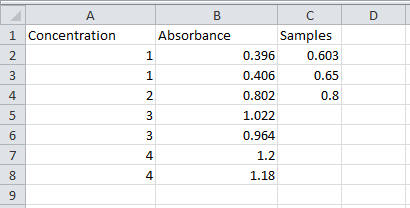
\includegraphics[width=0.6\textwidth]{img/excelscreen.PNG}
\caption{\label{fig:excel} De gebruikte excelsheet in dit voorbeeld. Opgeslagen als data.xlsx. }
\end{center}
\end{figure}

Een voorbeeld! We kunnen het Excelbestand in Fig \ref{fig:excel} importeren en weergeven met de volgende code:

\begin{lstlisting}[frame=single]
>>> data=pd.read_excel("data.xlsx")

>>> data
   Concentration   Absorbance  Samples
0               1       0.396    0.603
1               1       0.406    0.650
2               2       0.802    0.800
3               3       1.022      NaN
4               3       0.964      NaN
5               4       1.200      NaN
6               4       1.180      NaN
\end{lstlisting}

Een pandas DataFrame bestaat uit een verzameling van lijsten (daar heb je mee gewerkt in de vorige les). Elke lijst die je invoert is een rij en je kan elke rij een naam geven, wanneer je dat niet doet wordt deze automatisch genummerd te beginnen met 0.
Je kan ook zelf rechtstreeks data invoeren:

\begin{lstlisting}[frame=single]
>>> data=pd.DataFrame([[1, 2, 3], [4, 5, 6],[7, 8, 9]])

>>> data
   0  1  2
0  1  2  3
1  4  5  6
2  7  8  9

\end{lstlisting}
Wanneer je aan de kolomen een label wil geven doen je dat met "columns = []"

\begin{lstlisting}[frame=single]
>>> data = pd.DataFrame([[1,2,3],[4,5,6],[7,8,9]],columns = ['a', 'b', 'c'])

>>> data
   a  b  c
0  1  2  3
1  4  5  6
2  7  8  9

\end{lstlisting}
Een andere optie is een dictionary opgeven. \href{https://docs.python.org/2/tutorial/datastructures.html#dictionaries}{Officiele tutorial over dictionaries}.

\begin{lstlisting}[frame=single]
>>> data=pd.DataFrame({"a" : [1, 2, 3], "b" : [4, 5, 6], "c" : [7, 8, 9]})

>>> data
   a  b  c
0  1  4  7
1  2  5  8
2  3  6  9

\end{lstlisting}
Je ziet een aantal opvallende dingen. Zo heeft hij de 1e regel geimporteerd als namen van de kolommen (dat willen we graag!), is de eerste regel met data genummerd als regel 0 (net zoals met lijsten!) en zie je dat lege vakken worden gevuld met de text NaN. NaN staat voor "not a number" (=geen getal), en deze vakken zullen dus over worden geslagen bij berekeningen.
Een DataFrame kan meerdere typen data bevatten zoals, text, integers, floats en ook lege plekken, zoals je hierboven ook al hebt gezien. DataFrames zijn altijd 2D, dat wil zeggen dat ze altijd rijen en kolommen bevatten.

\section{Voorbeeld dataverwerking - Gamescores}
Noot: De complete tutorial vind je \href{https://www.dataquest.io/blog/pandas-python-tutorial/}{hier}, in het Engels, met plaatjes en extra uitleg. Hieronder een verkorte versie in het Nederlands. Voer de commando's zelf uit in Python om de output te zien. 

In dit voorbeeld gebruiken we een databestand die je hier kan downloaden: \href{http://www.sharecsv.com/s/3397aa3f9cf0cf20ae6c1428a32bfc07/ign.csv}{Klik!} 
Dit databestand bevat alle reviewscores die door website ign.com zijn toegekend. De dataset bevat verder nog meer info: welk platform de game op is gereviewed, in welk jaar, etcetera. Het is een .csv bestand, deze kan je ook importeren in Excel of SPSS. Met pandas kan je deze inlezen met de functie \textbf{read\_csv()}. Let op: het bestand wat je inleest moet in dezelfde directory staan als je pythonscript. Anders moet je het complete pad gebruiken. Daar moet je even opletten: gebruik dubbel slashes in het pad. In het voorbeeld zie je beide methodes:
\begin{lstlisting}[frame=single]
>>> import pandas as pd
>>> data = pd.read_csv("ign.csv") #lees bestand in
>>> data_complete_pad = pd.read_csv("C:\\Users\\Mok\\Downloads\\ign.csv") 
#gebruik hele pad als het niet goed werkt
\end{lstlisting}

We kunnen nu pandas vragen om een deel data netjes weer te geven. Voer de onderstaande code uit en je ziet als het goed is vanzelf wat de functies doen:
\begin{lstlisting}[frame=single]
>>> data.head(10) #eerste tien regels
>>> data.tail(7) #laatste 7 regels
>>> data.shape #aantal rijen en kolommen
(18625,11)
\end{lstlisting}

Het laatste commando geeft het aantal rijen en kolommen weer: er zijn dus meer dan 18000 reviews in dit bestand opgenomen, met 11 verschillende parameters per review. 

We kunnen ook wat statistiek doen:
\begin{lstlisting}[frame=single]
>>> data.mean()
>>> data.max()
>>> data.min()
>>> data.median()
>>> data.std()
>>> data.corr()
\end{lstlisting}

Je ziet dat pandas al deze functies op de hele dataset uitvoert. Je kan uiteraard ook individuele rijen of kolommen selecteren, of bijvoorbeeld kolom 1 t/m 5 van rij 1 t/m 100. Dit werkt eigenlijk hetzelfde als met lijsten, maar met iets andere commandos. Probeer het zelf (pas de cijfers aan en kijk wat er gebeurt!):
\begin{lstlisting}[frame=single]
>>> data.iloc[0:5,1]
>>> data.iloc[0:5,:]
>>> data.iloc[:,0:5]
>>> data.iloc[1,0:5]
>>> data.iloc[1:,:]
\end{lstlisting}

We kunnen zo dus ook de dataset opschonen. De eerste kolom bevat nutteloze info, dus laten we die weghalen:
\begin{lstlisting}[frame=single]
>>> data=data.iloc[:,1:] #eerste kolom weghalen
>>> data.head()  #checken of het goed is verwijderd
\end{lstlisting}

Dat werken met getallen is echter vaak niet handig. Nu moet je de hele tijd kijken welke rij ook alweer welke data had. Pandas maakt dat makkelijker voor je met labels. Je kan een naam koppelen aan een rij of kolom om zo makkelijk je data te selecteren. Dit zijn de namen die boven de kolommen staan in je data. Je kan dus bijvoorbeeld de volgende functies uitvoeren:
\begin{lstlisting}[frame=single]
>>> data.loc[0:5,"score"] #laat de kolom scores zien van rij 1 t/m 5
>>> data.loc[0:5,["score","release_year"]] 
#laat de score en uitgiftejaar zien van deze rijen
>>> data["score"] #laat de complete kolom score zien
\end{lstlisting}

Als we dus alleen geinteresseerd zijn in een deel van de info kunnen we dat selecteren. We kunnen ook filteren:
\begin{lstlisting}[frame=single]
>>> hoge_scores = data[data["score"]>7] 
#selecteer alle rijen waar de score hoger is dan 7
>>> hoge_scores.head(10)

>>> hoge_xbox_scores = hoge_scores[data["platform"] == "Xbox One"] 
#selecteer uit de lijst met hoge scores alle xbone games
>>> hoge_xbox_scores.head(10)
\end{lstlisting}

Het plotten van data kan ook. Je kan je bijvoorbeeld afvragen welk platform meer hoge scores krijgt: de PS4 of de XBOne?

\begin{lstlisting}[frame=single]
>>> import matplotlib.pyplot as plt
>>> ps4=data[data["platform"]=="PlayStation 4"] #alle ps4 data
>>> xbo=data[data["platform"]=="Xbox One"] #alle xbone data

>>> xbo["score"].plot(kind="hist") #plot alle xbox scores in een histogram
>>> plt.show() #laat de grafiek zien

>>> ps4["score"].plot(kind="hist") #plot alle ps4 scores in een histogram
>>> plt.show() #laat de grafiek zien
\end{lstlisting}

Als je de functies en hoe er mee om te gaan niet makkelijk kan onthouden: gebruik de cheat sheets die bovenaan het hoofdstuk staan. Dit zijn heldere overzichten van 1-2 A4 met alle belangrijke functies van pandas, numpy en matplotlib. Onthou: als je iets wil doen en je weet niet hoe: er is vast wel iemand die dat al een keer heeft geprobeerd, dus je kan in 9 van de 10 gevallen op internet gewoon het antwoord vinden. 

\textbf{A. Oefenen met pandas}
\begin{enumerate}[label=\textbf{A.\arabic*}]
\item Typ de dataset uit Fig~\ref{fig:excel} over in excel en sla op als data.xlsx. Importeer dit zoals uitgelegd in het hoofdstuk. Gebruik wat je hebt geleerd met pandas en voer een lineare regressie uit met de functie \textbf{linregress} uit het pakket \textit{scipy.stats}. \href{https://docs.scipy.org/doc/scipy/reference/generated/scipy.stats.linregress.html}{Hier de documentatie van linregress()}. 
\item Maak een plotje van de uitgevoerde lineare regressie (zie de link uit opdracht 3.1). Als het niet lukt: ga eerst verder met dit hoofdstuk, bij het deel matplotlib zal er meer info worden gegeven over het maken van plotjes.
\item Gebruik deze gegevens daarna om met behulp van een script de concentratie uit te rekenen van je samples. Als het niet lukt: ga googlen en je zal een heleboel uitgewerkte voorbeelden vinden! Als het niet lukt: ga eerst verder met dit hoofdstuk, bij het deel numpy zal meer info worden gegeven over het berekenen van data. 
\item BONUS: Pas je script aan zodat je het kan gebruiken met ieder willekeurig aantal meetpunten/samples. Maak er bijvoorbeeld een functie van die vanuit een XLSX of CSV direct de concentraties teruggeeft. De vorm van de data blijft altijd hetzelfde: eerst concentratie, dan absorbance, dan de samplewaardes.
\item Meer oefeningen vind je \href{https://github.com/ajcr/100-pandas-puzzles}{hier!}
\end{enumerate}

\section{Numpy}
\href{https://docs.scipy.org/doc/numpy/user/quickstart.html}{Officiele numpy tutorial}\\
\href{https://s3.amazonaws.com/assets.datacamp.com/blog_assets/Numpy_Python_Cheat_Sheet.pdf}{numpy Cheat Sheet}\\
\href{http://cs231n.github.io/python-numpy-tutorial/#numpy}{extra numpy-tutorial}\\
Numpy is een pakket waarmee je numpy-arrays kan maken en bewerken. Numpy-arrays zijn een speciaal soort lijsten, met veel ingebouwde functies. Als je wat geavanceerdere bewerkingen wil uitvoeren is dit pakket onmisbaar. Een numpy-array is direct te vergelijken met een matrix (zoals je bij wiskunde/lineaire algebra hebt gehad).
\\De belangrijkste verschillen tussen NumPy-arrays en Pandas-DataFrames zijn dat in NumPy-array maar \'e\'en type data kan staan, in tegenstelling tot Pandas-DataFrames waarbij je meerder typen data kan combineren. Waar Pandas-Dataframe altijd 2D is kunnen Numpy arrays veel meer dimensies hebben.

Het aanmaken van numpy arrays is simpel. Voer de onderstaande code uit en je ziet vanzelf wat er gebeurt:
\begin{lstlisting}[frame=single]
>>> import numpy as np
>>> a = np.array([1,2,3])
>>> a
>>> a[0]
>>> a[0:2]
>>> b = np.array([[1,2,3],[4,5,6]])
>>> b[0]
>>> b[0,0]
>>> b
\end{lstlisting}

In plaats van alle individuele getallen in de matrix te zetten zijn er ook functies om ze snel te maken. Probeer onderstaande code en kijk wat het maakt (en verander de getalletjes!):
\begin{lstlisting}[frame=single]
>>> a = np.zeros((5,5))
>>> b = np.ones((3,2))
>>> c = np.full((2,5),9)
>>> d = np.eye(5)
>>> e = np.random.random((4,3))
>>> f = np.arange(1,10,0.1)
\end{lstlisting}

Het opvragen van data uit een np-array gaat op dezelfde manier als uit lijsten: met slices.
Wanneer je een np-array sliced geeft het cijfer voor de komma het rijnummer aan en het cijfer na de komma de kolom. 
Probeer dit zelf ook uit met arrays met verschillende dimensies. Vergeet niet dat in python de nummering met 0 begint. Dus de eerste rij heeft rijnummer 0, de 2e rijnummer 1, etc.

\begin{lstlisting}[frame=single]
>>> a = np.random.random((4,4))

>>> a
array([[ 0.45423941,  0.02449346,  0.28748383,  0.86696254],
       [ 0.84538737,  0.88094837,  0.82634451,  0.46029926],
       [ 0.6649267 ,  0.23539764,  0.24480059,  0.40225708],
       [ 0.69317471,  0.70946337,  0.23112397,  0.45701743]])

>>> a[0,:]
array([ 0.45423941,  0.02449346,  0.28748383,  0.86696254])

>>> a[:,0]
array([ 0.45423941,  0.84538737,  0.6649267 ,  0.69317471])

>>> a[3,3]
0.45701742997293382

>>> a[0:2,2:4]
array([[ 0.28748383,  0.86696254],
       [ 0.82634451,  0.46029926]])
       
\end{lstlisting}

Net zoals in een pandas-array kan je ook data selecteren met behulp van voorwaarden:
\begin{lstlisting}[frame=single]
>>> a = np.array([1,2,3,4,5,6,7,8,9,10])
>>> b = a[(a>4)] #b=alle getallen groter dan 4 uit a
>>> c = a[(a%2==0)] #c=alleen even getallen uit a
\end{lstlisting}

we kunnen ook rekenen met arrays alsof het matrices zijn:
\begin{lstlisting}[frame=single]
>>> a = np.array([1,2,3,4,5,6,7,8,9,10])
>>> c=a*2
>>> b = np.full((1,10),3)
>>> d=a*b
>>> e=a/b
\end{lstlisting}

Kijk in de tutorials en de cheat-sheet voor meer handige en nuttige functies van numpy.

\textbf{B. Oefenen met numpy}
\begin{enumerate}[label=\textbf{B.\arabic*}]
\item Maak een functie die alle even getallen in een 1 bij X matrix negatief maakt.
\item Maak zelf een functie die uit een random matrix van 100x100 het hoogste getal teruggeeft. Gebruik de functie np.max om je antwoord te controleren.
\item als je meer wil oefenen, kijk dan \href{https://www.machinelearningplus.com/python/101-numpy-exercises-python/}{hier!}
\end{enumerate}

\section{Matplotlib}
\href{https://matplotlib.org/users/pyplot_tutorial.html}{Officiele matplotlib tutorial}\\
\href{https://s3.amazonaws.com/assets.datacamp.com/blog_assets/Python_Matplotlib_Cheat_Sheet.pdf}{matplotlib Cheat Sheet}

Matplotlib is een pakket om plotjes te maken. Om te beginnen heb je uiteraard eerst data nodig, deze data kan je importeren met pandas en bewerken met numpy, zoals je in de vorige paragrafen hebt geleerd.
Online is veel data verkrijgbaar een goede bron om mee te oefenen is de data van het cbs. 
\href{https://opendata.cbs.nl/#/CBS/nl/dataset/37221/table?dl=14447}{De data die gebruikt wordt voor de volgende voorbeelden kan je hier vinden.}
Stap 1 is het importeren van de data:

\begin{lstlisting}[frame=single]
>>> pd_uitstoot = pd.read_csv("C:/Emissies_naar_lucht_op_Nederlands_grondgebied__totalen_11112018_170037.csv")

>>> pd_uitstoot.head()
  Emissies naar lucht op Nederlands grondgebied; totalen
0                                                NaN    
1                                   ;"";"";"Bronnen"    
2  Onderwerp;"Perioden";"";"Totaal Stationaire en...    
3  CO2;"1990";"mln kg";"170410";"22080";"7550";"2...    
4  CO2;"1995";"mln kg";"180590";"17230";"7750";"2... 
\end{lstlisting}

Zoals je kan zien is het niet helemaal goed gegaan, dus zullen we eerst de data wat moeten opschonen.

\begin{lstlisting}[frame=single]
>>> pd_uitstoot = pd.read_csv("C:/Emissies_naar_lucht_op_Nederlands_grondgebied__totalen_11112018_170037.csv", skiprows = 3, sep = ";")

>>> pd_uitstoot.head()
  Onderwerp Perioden Unnamed: 2  Totaal Stationaire en mobiele bronnen  \
0       CO2     1990     mln kg                               170410.0   
1       CO2     1995     mln kg                               180590.0   
2       CO2     2000     mln kg                               182610.0   
3       CO2     2005     mln kg                               190780.0   
4       CO2     2010     mln kg                               198940.0   

   20-21 Chemie en farmaceutische industrie  24 Basismetaalindustrie  \
0                                   22080.0                   7550.0   
1                                   17230.0                   7750.0   
2                                   16470.0                   6360.0   
3                                   16280.0                   7240.0   
4                                   18200.0                   6890.0   

   Particulier huishouden  01 Landbouw (stationaire bronnen)  Vervoer  \
0                 22350.0                             7750.0  29860.0   
1                 25030.0                             8260.0  31710.0   
2                 22320.0                             7500.0  35660.0   
3                 21710.0                             7440.0  37810.0   
4                 25350.0                            10190.0  37780.0   

   Railverkeer  Wegverkeer  Scheepvaart  Luchtvaart  
0         90.0     23980.0       5470.0       320.0  
1         90.0     25570.0       5600.0       450.0  
2        110.0     28290.0       6640.0       610.0  
3        110.0     29910.0       7110.0       680.0  
4        110.0     29960.0       7040.0       670.0  

\end{lstlisting}

Nu we de data in een pandas DataFrame hebben staan kunnen we de data opschonen. De laatste rij bevat een hoop NaN. Met df.dropna() worden alle rijen waar NA (not available) of NaN (not a number) staat verwijderd.

\begin{lstlisting}[frame=single]
>>> pd_uitstoot = pd_uitstoot.dropna()
\end{lstlisting}

Wanneer we de uitstoot van railverkeer en luchtvaart met elkaar willen vergelijken kunnen we deze op verschillende manieren in een plot weergeven. Hieronder een voorbeeld:

\begin{lstlisting}[frame=single]
>>> pd_uitstoot["Perioden"][8] = 2017

>>> x = pd_uitstoot["Perioden"]

>>> y = pd_uitstoot["Railverkeer"]

>>> plt.scatter(x, y, label = "Railverkeer")
<matplotlib.collections.PathCollection object at 0x0000000004F36C88>

>>> z = pd_uitstoot["Luchtvaart"]

>>> plt.scatter(x, z, label = "Luchtvaart")
<matplotlib.collections.PathCollection object at 0x0000000004F5E1D0>
>>> plt.show()
\end{lstlisting}

Het plotje komt er dan uit te zien zoals in Fig. ~\ref{fig:matplotlib_scatter_1}

\begin{figure}[h]
\begin{center}
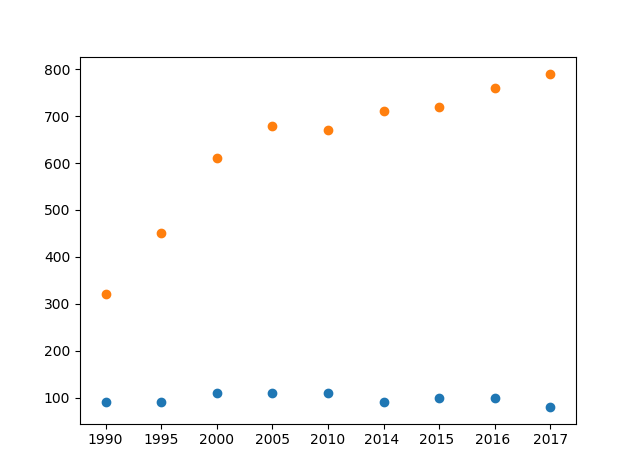
\includegraphics[width=0.6\textwidth]{img/matplotlib_scatter_1.png}
\caption{\label{fig:matplotlib_scatter_1} Scatterplot van de uitstoot railverkeer en luchtverkeer per jaar}
\end{center}
\end{figure}

Zonder labels en legenda is deze plot niet compleet, dus laten we die toevoegen!

\begin{lstlisting}[frame=single]
>>> plt.xlabel("Jaar")
Text(0.5,0,'Jaar')

>>> plt.ylabel("mln kg")
Text(0,0.5,'mln kg')

>>> plt.legend()
<matplotlib.legend.Legend object at 0x00000000086C5BE0>

>>> plt.show()

\end{lstlisting}

Met labels komt het de grafiek er dan uit te zien als Fig.~\ref{fig:matplotlib_scatter_2}.

\begin{figure}[h]
\begin{center}
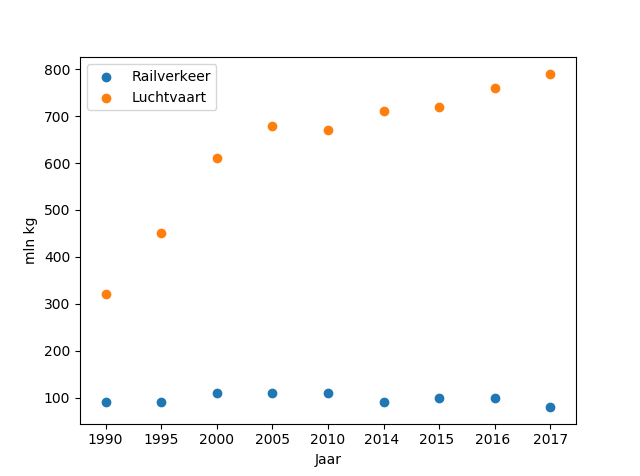
\includegraphics[width=0.6\textwidth]{img/matplotlib_scatter_2.png}
\caption{\label{fig:matplotlib_scatter_2} Scatterplot van de uitstoot railverkeer en luchtverkeer per jaar met labels}
\end{center}
\end{figure}

\textbf{C. Oefenen met Matplotlib}

\begin{enumerate}[label=\textbf{C.\arabic*}]
\item Maak een plot van de ign.csv data met behulp van matplotlib. Kies zelf wat je wil plotten. Selecteer de data met behulp van pandas, en maak de plot mooi met matplotlib. 
\item Meer oefeningen vind je \href{https://www.w3resource.com/graphics/matplotlib/}{hier!}
\end{enumerate}


